\documentclass{jarticle}

\usepackage[dvipdfmx]{graphicx}
\usepackage{float}
\usepackage{url}

\title{光速度の測定}
\author{2511198 肥田幸久 \\ 共同実験者 \\ 2511238 矢吹千陽}
\date{2025年5月29日作成}

\begin{document}
\maketitle



\section{実験の目的}
光速度は物理学のもっとも基本的かつ重要な定数のひとつであり, 1983年から国際単位系(SI)の$\mathrm{m}$の定義は, 真空中における光速度を基準として定めている. そのため光速度の性格な測定は極めて重要な意味を持つ.

本実験ではこの光速度と, それに加えて同軸ケーブルを伝わる信号の速度の測定を行う.



\section{実験の原理}


\subsection{光速度の測定}

光速度の測定には, 木星の衛星の食, 光行差, 回転歯車, 回転鏡など歴史的にさまざまな方法が用いられてきた. 本実験では, それらに比べてシンプルかつ直接的な方法である「距離と時間の差」により、光速度を測定する.

光速度$c$は, 距離$d$を光が移動するのにかかる時間$t$を用いて,
\begin{equation}
  c=\frac{d}{t}
\end{equation}
と表される. この関係は本実験のもっとも根本的な原理である.

本実験では, 同一のパルスレーザー光を短距離経路と長距離経路に分岐させ, それぞれの往復にかかる時間を比較する. 両者の時間差$T$と光路差$L$を用いて光速度$c$は以下のように表される.
\begin{equation}
  c=\frac{L}{T}
\end{equation}
これにより, 絶対的な時間や距離を測定することなく, 高精度な光速度の測定が可能となる.


\subsection{同軸ケーブルを伝わる信号速度の測定}

パルス発生器から半導体レーザーに接続されている同軸ケーブルをインピーダンス整合器ごと取り外すと, インピーダンスの整合がとれないため終端で信号パルスが反射する.

この実験では, パルス発生器から直接観測したパルスと終端の反射によって生じたパルスとの時間間隔$T$を測定する.
このパルスの時間間隔$T$と同軸ケーブルの長さを$L$を用いて, 同軸ケーブルを伝わる信号速度$v$は以下のように表される.
\begin{equation}
  v=\frac{2L}{T}
\end{equation}



\section{実験方法}


\subsection{光速度の測定}

本実験では図\ref{fg:lightspeed-method}のような装置を用いて測定を行った.
図中の半導体レーザー(レーザーダイオード)は波長$685\,\mathrm{nm}$の赤色光を出す.
そこでパルス発生器からレーザーに電圧を加え, 幅約$10\,\mathrm{ns}$の光パルスを出力させる.
この短い光パルスを観測するために, 応答時間が$1\,\mathrm{nm}$以下の光検出器, ここではpinフォトダイオード(pin接合のダイオード)を使用する.

\begin{figure}[H]
  \begin{center}
    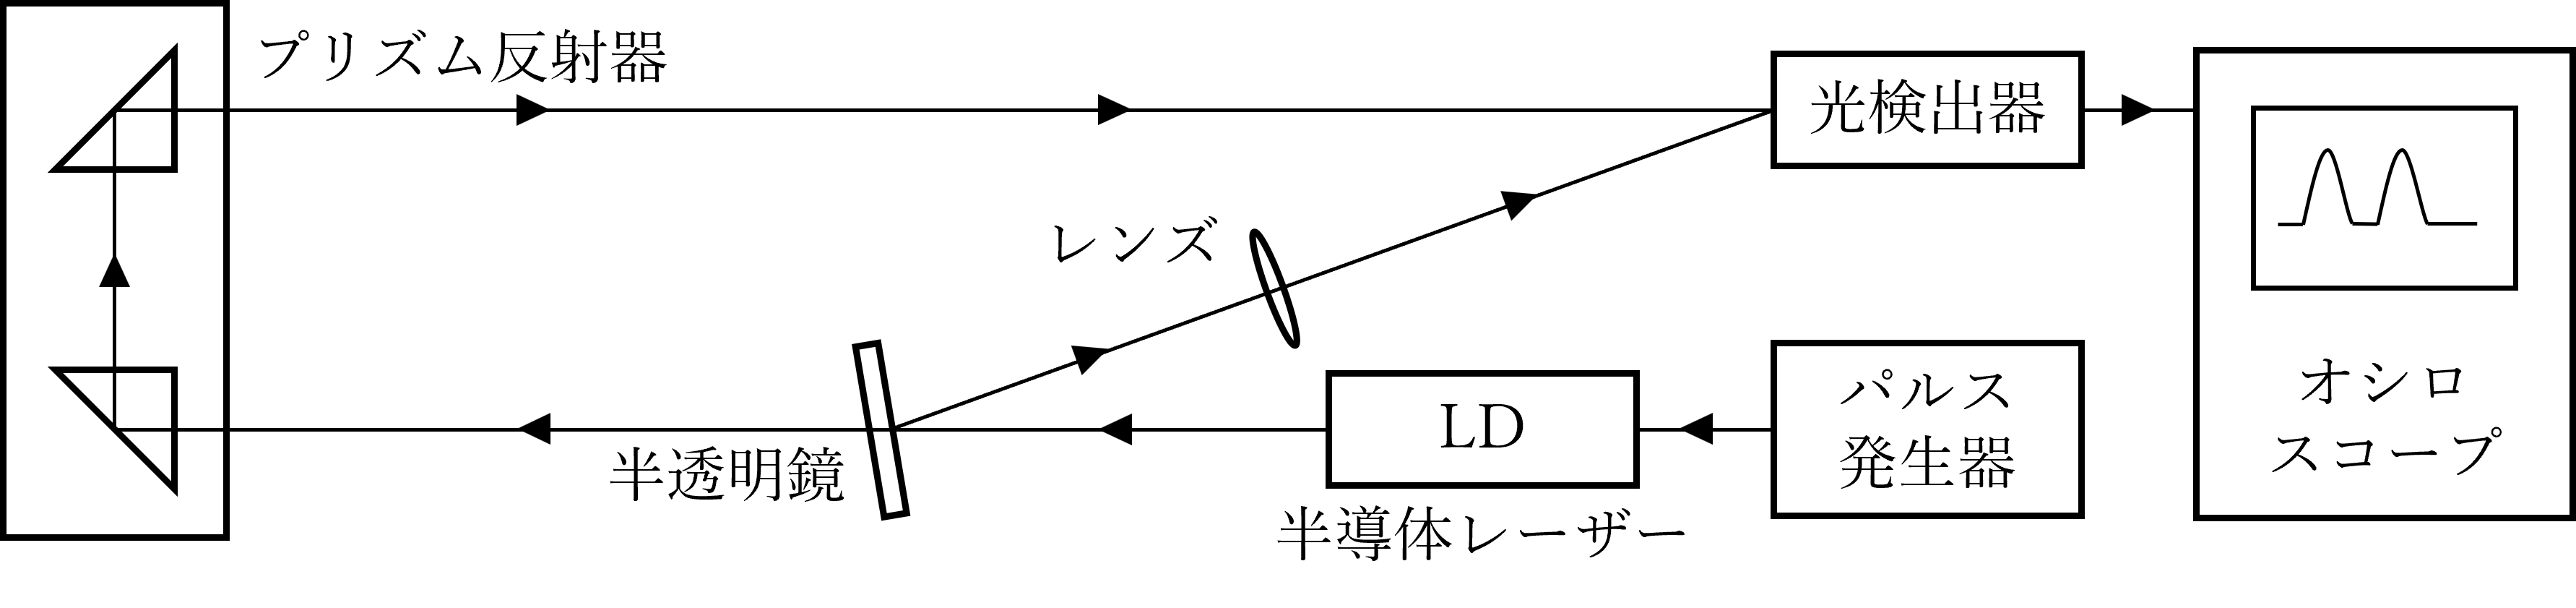
\includegraphics[width=110mm]{experimental_method_picture.png}
    \caption{光速度の測定装置}
    \label{fg:lightspeed-method}
  \end{center}
\end{figure}

測定では, 半導体レーザーから繰り返し周波数約$15\,\mathrm{MHz}$の光パルスを数$\mathrm{m}$離れたプリズム反射器で反射させて光検出器に導く.
また, 半導体レーザーとプリズム反射器の間でレーザーの一部を半透明鏡で反射させ, 同じ光検出器に導く.

光検出器の出力信号をオシロスコープに導き, 2つの光パルスの時間間隔$T$を測定する.
加えて, プリズム反射器を通じて光検出器に入る光路(長距離経路)と, 半透明鏡を通じて光検出器に入る光路(短距離経路)との差$L$を図\ref{fg:lightspeed-distance}のように測定する.

\begin{figure}[H]
  \begin{center}
    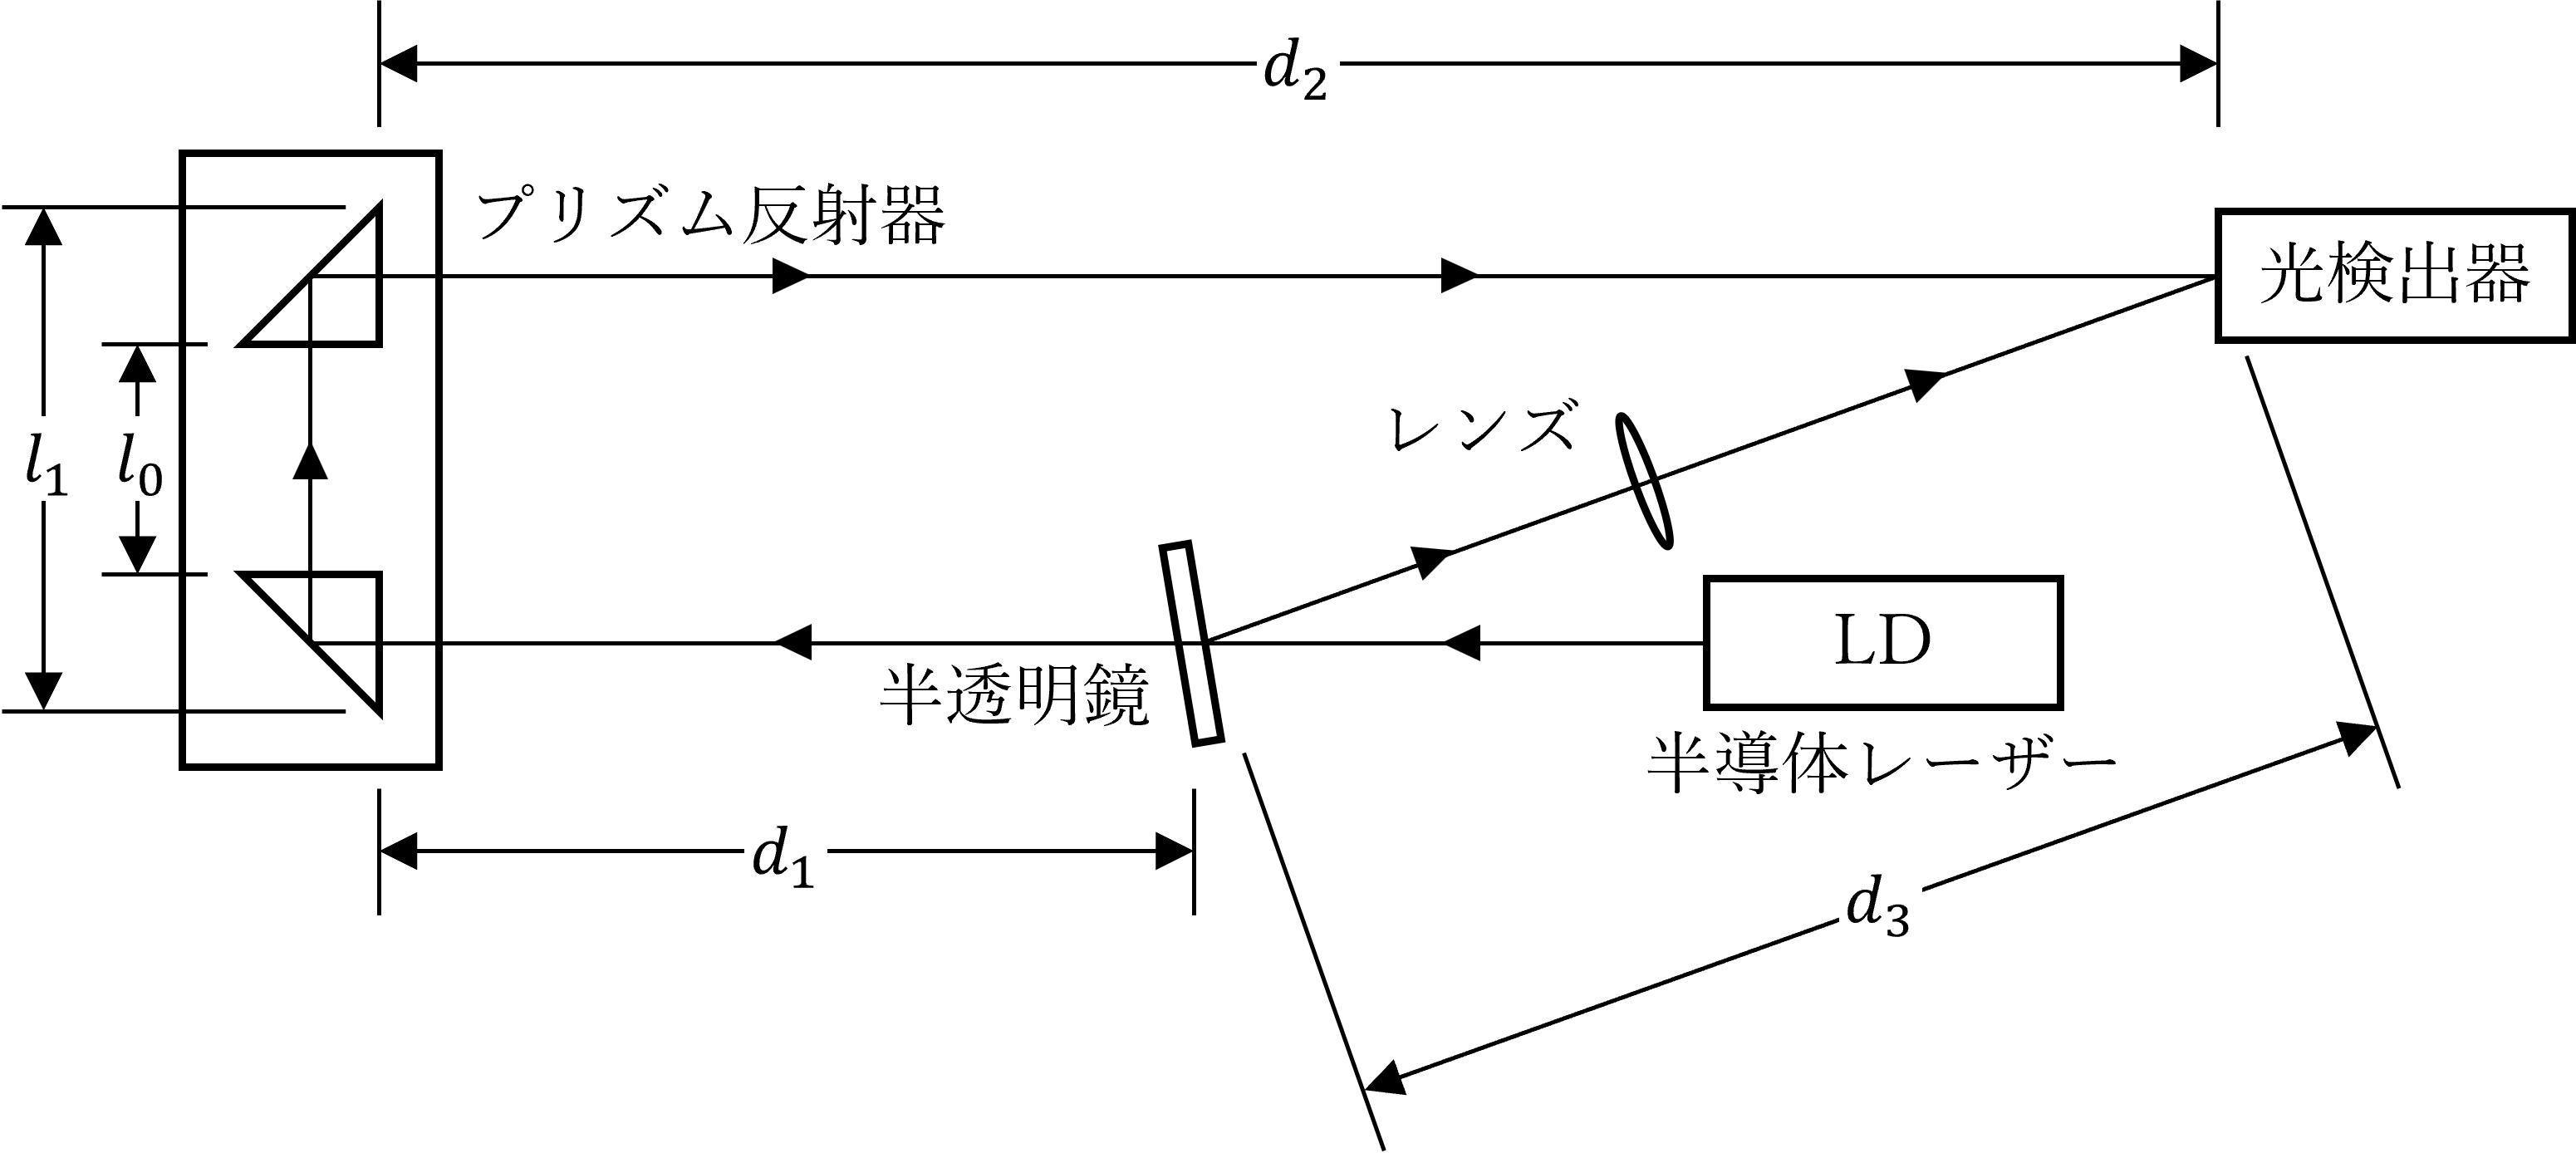
\includegraphics[width=95mm]{experimental_distance_picture.png}
    \caption{光路の測定}
    \label{fg:lightspeed-distance}
  \end{center}
\end{figure}

プリズムのガラスの屈折率を$n$とすると, 光路差$L$は次の式(\ref{eq:L})で求められる.
\begin{equation}
  \label{eq:L}
  L=d_1+d_2-d_3+n(l_0-l_1)+l_1
\end{equation}


\subsection{同軸ケーブルを伝わる信号速度の測定}




\section{実験結果}


\subsection{光速度の測定}

次の表\ref{tb:lightspeed-distance}に, 光路の測定結果を示す.

\begin{table}[h]
  \centering
  \caption{光路の測定結果}
  \begin{tabular}{cccccc}
    \hline
    回数 & $d_1/\mathrm{mm}$ & $d_2/\mathrm{mm}$ & $d_3/\mathrm{mm}$ & $l_0/\mathrm{mm}$ & $l_1/\mathrm{mm}$ \\
    \hline
    1 & 2380.0 & 2864.5 & 520.5 & 177.2 & 128.2 \\
    2 & 2381.5 & 2873.0 & 522.5 & 178.1 & 128.6 \\
    3 & 2376.2 & 2872.1 & 521.2 & 178.8 & 128.8 \\
    \hline
    平均 & 2379.2 & 2869.9 & 521.4 & 178.0 & 128.5 \\
    \hline
    \label{tb:lightspeed-distance}
  \end{tabular}
\end{table}

この光路の測定結果より, 光路差$L$は式(\ref{eq:L})より求められる.
実験で使用した直角プリズムの材料をBK7と仮定すると, \cite{Glass-Materials}より屈折率は$n=1.513$となる.
これを用いて計算すると$L=4931.1\,\mathrm{mm}$と求められる.

次に, 今回の実験で観測したオシロスコープの画面を以下の図\ref{fg:lightspeed-oscilloscope}に示す.

\begin{figure}[H]
  \begin{center}
    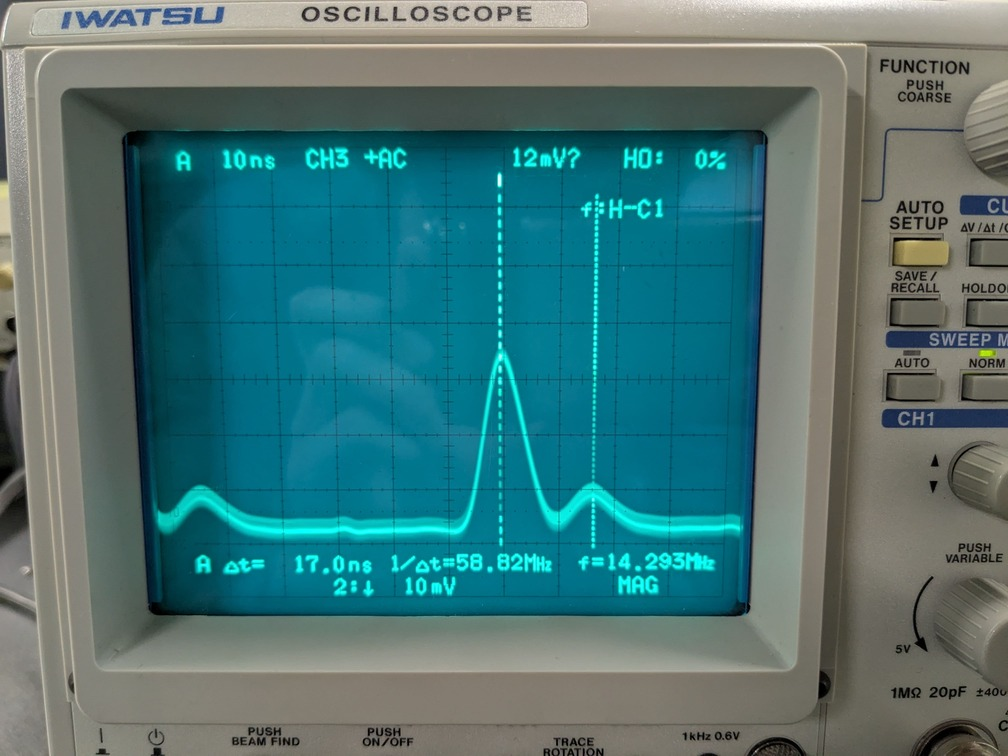
\includegraphics[scale=0.3]{lightspeed_result_picture.jpg}
    \caption{光速度の測定におけるオシロスコープの画面}
    \label{fg:lightspeed-oscilloscope}
  \end{center}
\end{figure}

これより, パルスの時間間隔$T=17.0\,\mathrm{nm}$と測定できた.
よって光路差$L$とパルスの時間間隔$T$より, 光速度$c$の測定結果を次の表\ref{tb:lightspeed-result}に示す.

\begin{table}[h]
  \centering
  \caption{光速度$c$の結果}
  \begin{tabular}{ccccc}
    \hline
    $L/\mathrm{mm}$ & $T/\mathrm{ns}$ & $c/\mathrm{ms^{-1}}$ & 文献値\cite{light-speed} & 誤差 \\
    \hline
    4931.1 & 17.0 & $2.901\times10^8$ & $2.998\times10^8$ & $-0.097\times10^8$ \\
    \hline
    \label{tb:lightspeed-result}
  \end{tabular}
\end{table}



\subsection{同軸ケーブルを伝わる信号速度の測定}

以下に今回の実験で観測したオシロスコープの画面および同軸ケーブルの長さを示す.

\begin{figure}[H]
  \begin{center}
    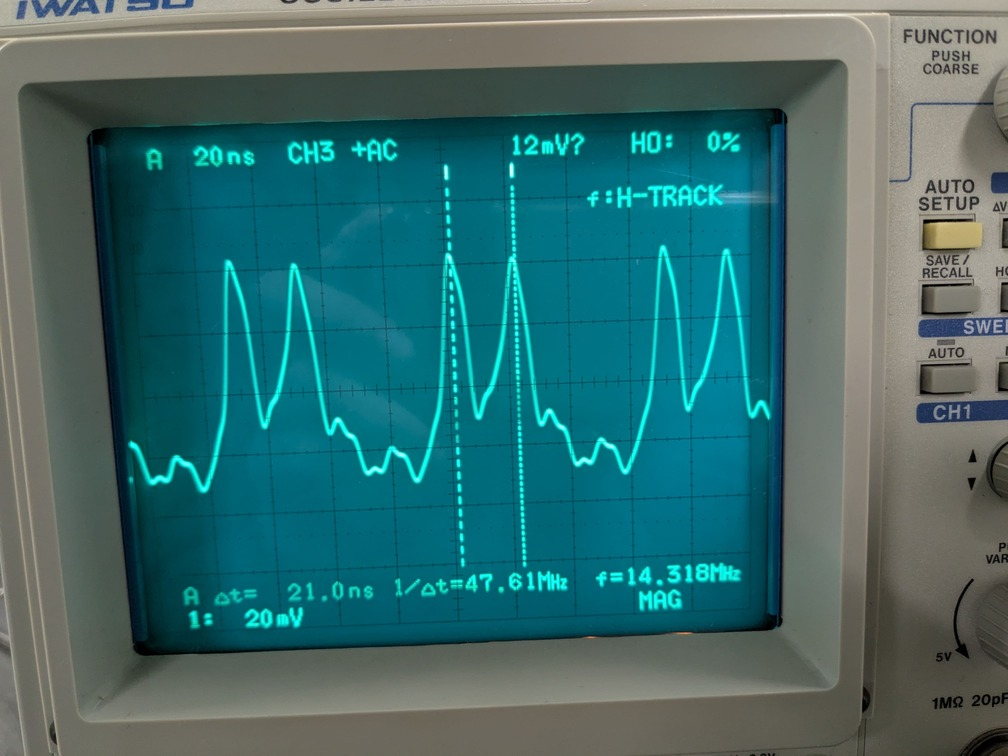
\includegraphics[scale=0.3]{cable1_result_picture.jpg}
    \caption{$L=2.04\,\mathrm{m}$}
  \end{center}
\end{figure}

\begin{figure}[H]
  \begin{center}
    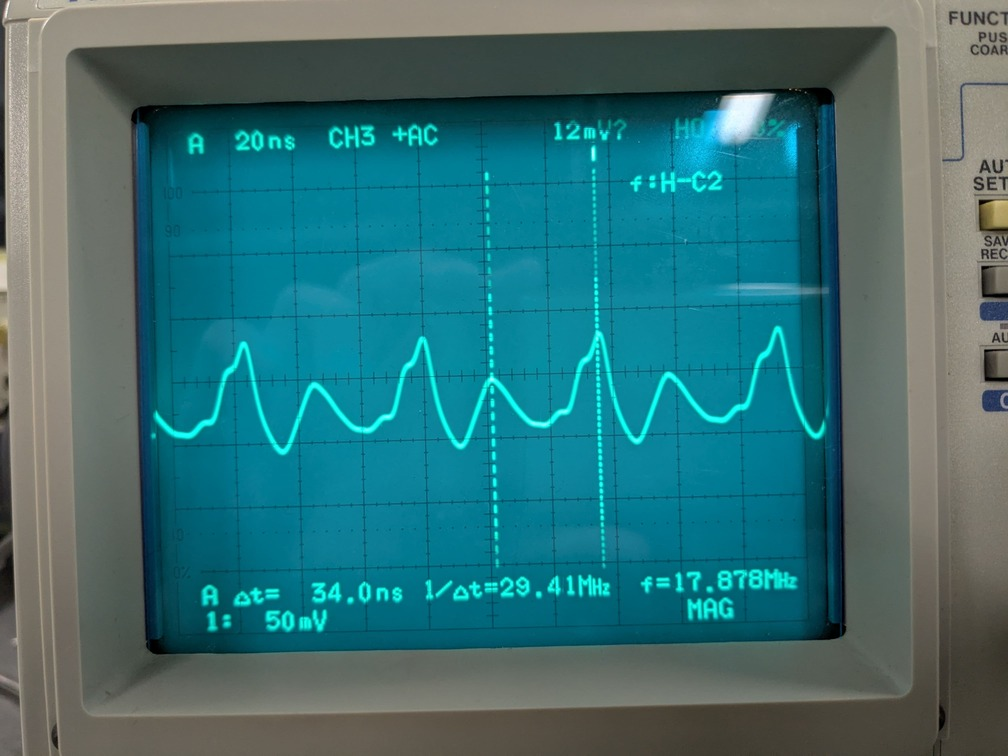
\includegraphics[scale=0.3]{cable2_result_picture.jpg}
    \caption{$L=7.61\,\mathrm{m}$}
  \end{center}
\end{figure}

\begin{figure}
  \begin{center}
    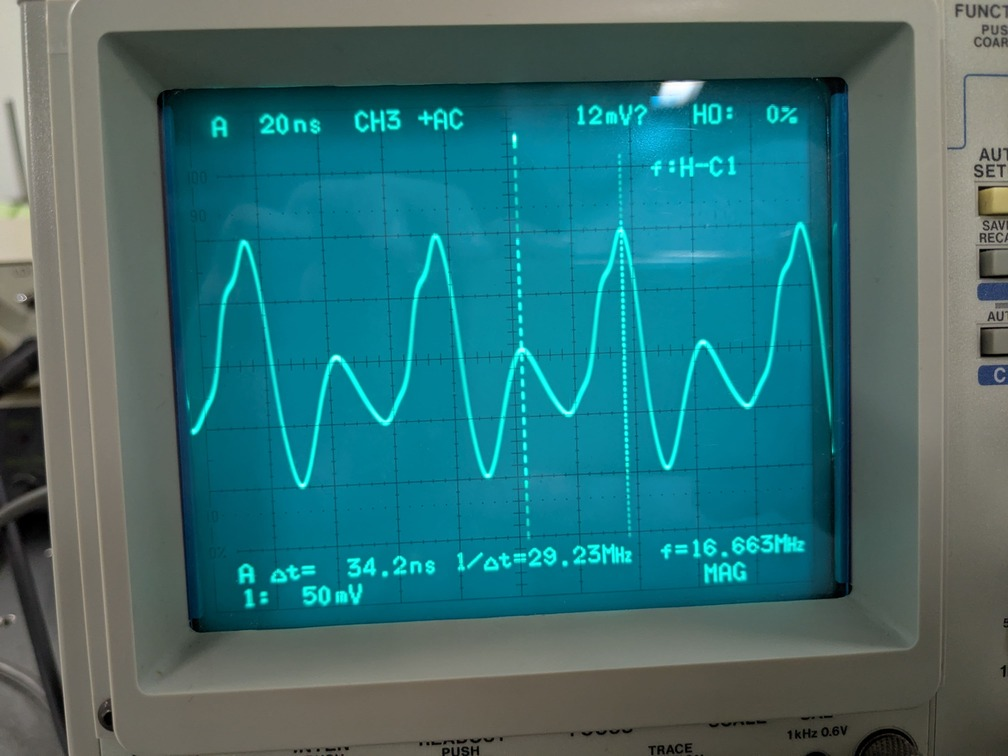
\includegraphics[scale=0.3]{cable3_result_picture.jpg}
    \caption{$L=5.06\,\mathrm{m}$}
  \end{center}
\end{figure}

\begin{figure}[H]
  \begin{center}
    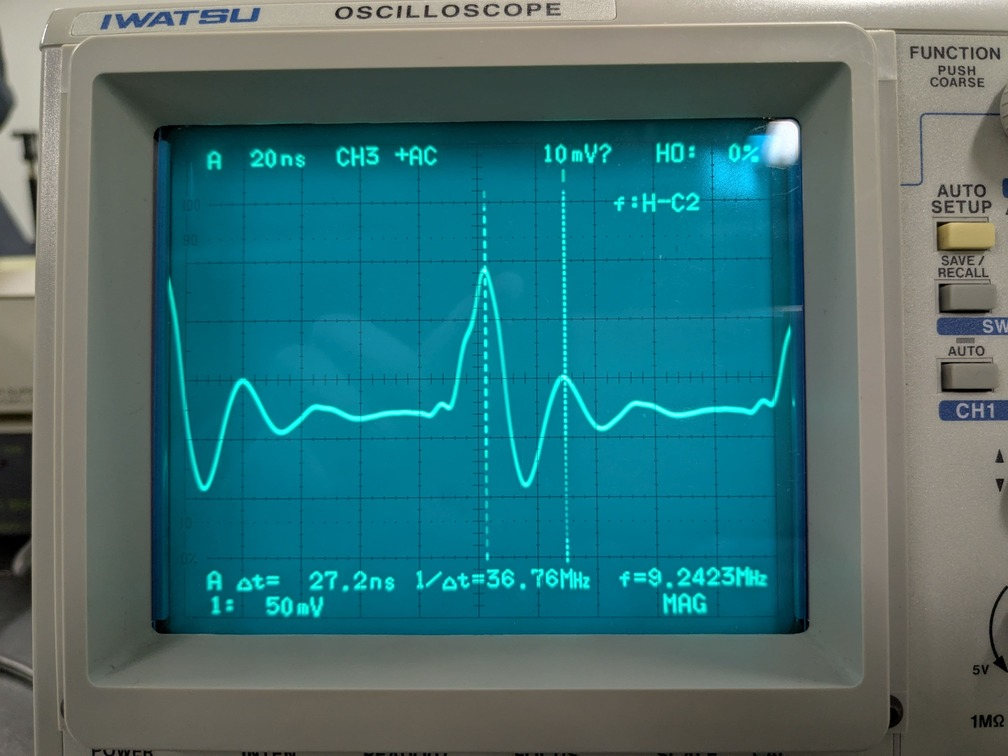
\includegraphics[scale=0.3]{cable4_result_picture.jpg}
    \caption{$L=10.03\,\mathrm{m}$}
  \end{center}
\end{figure}

\begin{table}[h]
  \centering
  \caption{同軸ケーブルを伝わる信号速度の測定結果}
  \begin{tabular}{ccccc}
    \hline
    ケーブル & $L/\mathrm{m}$ & $T/\mathrm{ns}$ & $v/\mathrm{ms^{-1}}$ \\
    \hline
    1 & 2.04 & 21.0 & $1.94\times10^8$ \\
    2 & 7.61 & 34.0 & $4.48\times10^8$ \\
    2 & 5.06 & 34.2 & $2.96\times10^8$ \\
    4 & 10.03 & 27.2 & $7.38\times10^8$ \\
    \hline
  \end{tabular}
\end{table}



\section{考察}


\subsection{空気の屈折率}

大気圧, 室温における空気の屈折率は$n=1.00028$であるが, これが今回の実験で測定した空気中の光速度について, "空気中"であって"真空中"ではないことを問題とすべきか考察する.

空気の屈折率$n=1.00028$より, 空気中の光速度は真空の光速度と比較して0.028\%低下する.
これは今回の実験で求めた光速度$2.901\times10^8\,\mathrm{ms^{-1}}$と比較すると十分に小さいため, 空気の屈折率を問題にする必要はない. もちろん, より高精度を求められる測定の際には, 空気の屈折率による影響を考慮する必要がある.


\subsection{同軸ケーブルの信号速度}

今回の実験では, 同軸ケーブルを伝わる信号速度の測定結果の値がケーブルごとに大きく異なっていた.
原因としては, パルスの時間間隔すなわちオシロスコープの使い方に問題があったのではないかと考え, 仮説を2つ挙げることにする.

1つ目は, 波形の読み間違いである.
今回の実験では, 波形を観察するために, オシロスコープおよびパルス発生器の設定を大きく変更していた.
これによって例えば周期を超えてパルスの遅れを観察してしまうなどのミスが起きたのではないかと考える.

2つ目には, 前述したとおり, オシロスコープおよびパルス発生器の設定を大きく変更していたために, 本来の関係ない波形の動きを増幅させてそれを観察してしまった可能性もあると考える.



\begin{thebibliography}{99}

  \bibitem{Glass-Materials}
  シグマ光機株式会社, ガラス材料 \url{https://jp.optosigma.com/ja_jp/category__opt_d__opt_d01}

  \bibitem{light-speed}
  山形大学, 真空中の光速度, \url{https://edu.yz.yamagata-u.ac.jp/developer/Asp/Youzan/Physics/Quantity/@Quantity.asp?nQuantityID=102}

  \bibitem{cable}
  電子コンポーネント(株), 同軸ケーブルの基本の概要, \url{https://www.ic-components.jp/blog/overview-of-coaxial-cable-basics.jsp}

\end{thebibliography}


\end{document}